\documentclass[msc]{ppgccufmg}    % ou [msc] para dissertações
                                  % de mestrado. Para propostas ou
                                  % projetos, usar [phd,project],
                                  % [msc,proposal], etc.

%\usepackage[brazil]{babel}        % se o documento for em português, OU
\usepackage[english]{babel}      % se o documento for em inglês
\usepackage[utf8]{inputenc}
\usepackage[T1]{fontenc}
\usepackage{type1ec}
\usepackage{amsmath,amssymb,amsthm}
\usepackage{graphicx}
\usepackage{multirow}
\usepackage{tikz}
\usepackage{subcaption}
\usepackage[export]{adjustbox}
\usetikzlibrary{arrows.meta}
\usepackage[
  portuguese,
  bookmarks=true,
  bookmarksnumbered=true,
  linktocpage,
  colorlinks,
  citecolor=black,
  urlcolor=black,
  linkcolor=black,
  filecolor=black,
  ]{hyperref}
\usepackage[square]{natbib}
\bibliographystyle{unsrtnat}
\usepackage{url}
\usepackage{indentfirst}

\newtheorem{mydef}{Definition}
\newtheorem{myprop}{Proposition}
\newtheorem{myred}{Reduction}
\newtheorem{mylemma}{Lemma}
\newtheorem{mytheo}{Theorem}
\newtheorem{myproof}{Proof}



\begin{document}
\ppgccufmg{
  title={Integer Formulation for Target Set Selection },
  authorrev={Rasador Panizzi, Alana},
  cutter={D1234p},
  cdu={519.6*82.10},
  university={Universidade Federal de Minas Gerais},
  course={Computer Science},
  address={Belo Horizonte},
  date={2019-09},
  keywords={Graphs, Networks, Spread Infection, Dynamic Monopolies, Influence Spreading, Spread of Information,Viral  Marketing},
  advisor={Sebasti\'an Alberto Urrutia\\ Vin\'icius Fernandes dos Santos},
%  approval={img/approvalsheet.eps},
%  approval=[-2.5cm][1]{aprovalsheet},
%  abstract={Resumo}{resumo},
 % abstract=[english]{Abstract}{extra/Abstract},
%  abstract={Resumo Estendido}{resumoest},
% dedication={extra/Dedication},
%  ack={agradecimentos},
% ack=[Acknowledgments]{extra/Acknowledgments},
epigraphtext={But I've never seen the Icarus story as a lesson about the limitations of humans. I see it as a lesson about the limitations of wax as an adhesive.}{Randall Munroe},
 %indexkeys={1. Computer Science}
  }
  
  \chapter{Introduction}

Propagation of diseases through the population, fake news through social networks, or even failures through distributed networks: These are some examples of irreversible conversion processes, which simulate the dissemination of a certain characteristic in a subset of the vertices in a graph, that in turn pass such characteristic on to the others vertices, and so on. 
This problem has already been studied under various names in various areas of computer science, being versatile and applicable to the most varied fields.

Given that each vertex in this graph has a resistance to infection, we will be mainly interested in the problem of minimum convergent set, or target set selection, which aims to find the minimum subset of vertices of a graph, such that if the vertices of the set are initially infected, then they will carry on the infection to all other vertices. The decision version of this problem with the most simple spreading rule was shown to be NP-complete in \cite{dreyer2009}.

In the literature, we have few integer models that attempt to solve exactly this problem, and based on this we believe that much can be contributed to the area by providing other formulations for this problem.  

%<insert here summary of next chapters>
%<make better introduction when finish text>

\section{Motivation}
Irreversible conversion processes are widely studied in the most diverse areas, and have the most varied practical applications. As we see in \cite{kutten1999}, as communication networks grow, existing fault-handling tools that involve time measurements, such as global wait times or resetting procedures, become increasingly inaccessible, since its cost grows with the size of the network. Therefore, for a fault-handling mechanism to scale to large networks, its cost now depends only on the number of failed nodes. Finding the minimum number of vertices that leads to the compromise of the network as a whole is one of the applications of the problem studied here.

In addition, different processes with economic and social implications can be modeled as irreversible conversion processes. Given a graph that models the social interaction between individuals, it can be said that the behavior of each individual is influenced by their direct neighbors. Many companies are interested in the minimal group of individuals who most influence a social network in order to focus resources and efforts to efficiently market their products.

Another way in which we encounter this problem is in the process of disseminating ideas and opinions in a group of people. \citeauthor{dreyer2009} give the example of finding the most influential subgroup in the group, that is, the set of individuals who, if they agree with an opinion or idea at the beginning of the process, guarantee that the group will eventually also agree. Finding the smallest group of these individuals can have both social applications in public awareness campaigns for example as well as economic ones, helping companies to modify or influence the consumer's view of their brand (rebrand).

These are just some of the applications of irreversible conversion processes that show how modeling and solving this problem has great economic and social value.


\section{Goals/Overview}

%Because it is an NP-complete problem, we will approach the problem with integer programming, using a simple direct integer model as a starting point. We want to find improvements, or even an alternative and more efficient way to represent the problem, and we can use models based on different interpretations from those proposed here. In addition, the starting entire model can be greatly improved by inequalities and lower boundaries that reduce the solution space. Taking this into account, it is important to study problem-specific structures. It is important to focus on this part of the problem solving, because for some very important graph classes the problem cannot be solved in a timely manner.

%Study the best heuristics that can help solving our problem for helping branch-and-cut approaches, since relying on exact solutions provided by the solvers can be extremely inefficient. 
Breafly, our mail goals in this dissertation was to:
\begin{itemize}
\item Review the literature regarding the Target Set Selection Problem and gather all current relevant results for this problems, which is challenging, since this problem appears under many different names, depending on the area it was being studied;
\item Describe current integer formulations in the literature that will be relevant to our work with more detail, as well as a starting very simple model, build directly from the problem definition;
\item Describe the new paradigm used to define our integer model, proving the core properties we use in our formulation; 
\item Show the branch and cut algorithm created, but consequently show its limitations when proving the separation problem to be NP-complete; 
\item Since our separation problem is so difficult, study which strategies can be tried in order to execute our branch-and-cut algorithm in timely manner. 
\item Present experimental results that compare our new model to the formulations in the literature.
\end{itemize}


\chapter{Literature review}
As we see in \cite{dreyer2009}, modeling attempts that describe how infectious diseases spread can be traced back to Bernoulli in 1760 in smallpox studies. Nowadays, based on dynamic systems models, these are still being analyzed. However, another interesting way to address such a problem is to note that diseases are spread through social networks, which can be very well represented by graphs.
Another problem very close to that of spreading diseases is the spreading of opinions in social networks, as well as of faults in computer networks. These have ample literature, as we can see in some of the early articles in these areas: \cite{poljak1983}, \cite{degroot1974} and \cite{french1956}.

According to \cite{dreyer2009}, the problem of irreversible conversion processes is defined as a model where given a $ G = (V, E) $, $ V $ being the set of vertices and $ E $ the set of edges, and each vertex $ v_{i}$ is in a state $ x_{i} ={0, 1}$ at a given time instant $ t $. The process is said irreversible because when a vertex enters the $ 1 $ state, or also said "infected", it will remain infected in the rest of the process.
The goal of this paper, however, is to characterize irreversible processes, where, in addition to being irreversible, each vertex assumes state 1 from state 0 if at least $ k $ of its neighbors are already infected. To find the smallest set of vertices, called the irreversible conversion set k, in which all the vertices of this set are infected at the beginning of the process, and in the end, will lead to the infection of all the vertices of the graph, shown to be an NP- complete for any $ k $ greater than 2. In sequence, \cite{chen2009} show the NP-completeness of the problem for $ k = 2 $, responding to the open conjecture proposed by \citeauthor{dreyer2009}.

In addition to proving the conjecture, \citeauthor{centeno2011} also show results for a generalization of the above-mentioned problem. In this more general form of the problem, the number of infected neighbors required for vertex infection is modeled by any function $ f: V \rightarrow \mathbb{Z} +$, instead of the previously used constant $ k $ , being denoted by $ irr_{f} (G) $. The results obtained in this paper describe a general reduction principle for $ irr_{f} (G) $, which leads to efficient algorithms for graphs with simple structure blocks, such as trees and chordal graphs.

In the article \cite{chopin2014}, the problem is called \textit{Target Set Selection}, and we see that in addition to generalizing the irreversible conversion set k, $ irr_{f} $ generalizes others problems in well-known graphs, such as Dominating Set with thresholds in \cite{Cordasco2018}, Vector Dominating Set in \cite{Cicalese2013}, K-Tuple Dominating Set \cite{Liao2003}, Vertex Cover, where the threshold function describes the degree value of each vertex and proved in \cite{chen2009}, r-Neighbor Bootstrap Percolation in \cite{balogh2009}, and dynamic monopolies in \cite{Khoshkhah2012}.

In \cite{Reddy2010} we see that for the class of bipartite graphs, the problem is NP-complete, but for the tree classes,
clicks, complete split graphs, threshold graphs and chain graphs, polynomial algorithms were found. Also studied as Target Set Selection, this problem is shown in \cite{BenZwi2009} to be $n^{\mathcal{O}(w)}$ with $n$ and $w$ being respectively the number of vertices and the graph's\textit{ treewidth}, which roughly measures the degree in which a given graph is similar to a tree in a very deep structural sense. This helps us to see how this problem will probably behave in instances where the graph is farther from a tree.

\citeauthor{Ackerman2010} also show a few extra bownds for this problem. Their upper bound implies that there are always Perfect Target Sets, the minimun set of initial infected vertices that infects the whole graph,  of size at most $|V|/2 $ and $ 2|V|/3$ under majority  $f(v)=\lceil deg_{in}(v)/2 \rceil $ and strict majority $f(v)=\lceil (deg_{in}(v) + 1)/2 \rceil$ thresholds . They also define a combinatorial model for the Target Set Selection problem relying on the idea that finding a way of directing the graph edges forming a directed acyclic graph, similarly to the way the infection spreads throw out the graph, respecting the rule where the infection only spreads if the vertex has sufficient edges pointing to it.  Unfortunately, this paper does not present experimental results for this model, making it difficult to compare our model to it. 

When we look for works in the experimental area of irreversible conversion processes, we realize that these are very scarce in the literature.\citeauthor{amaral2015} uses genetic algorithms to find results for the minimal convergent set problem seen here and, in \cite{Soltani2019}, we have a model based on \citeauthor{Ackerman2010}'s model,  where both are compared in the paper's experimental results. We will compare our model against \citeauthor{Soltani2019} models, since the code and instances are more easily accessible, and seem to show concrete results against the already well stablished model presented by \citeauthor{Ackerman2010}.


The version of the problem with the threshold function $ f (v, t) $ that changes over time and adds a maximum time-out for the total infection of the graph is seen in \cite{rautenbach2014}. In this article, we see that if G is a forest or a click, \citeauthor{rautenbach2014} presents efficient algorithms that compute $ irr (G, t_d, f) $. In addition, upper and lower bounds are tested based on counting and probabilistic arguments. For the special choices of $ t_d $ and $ f $, the parameter $ irr (G, t_d, f) $ coincides with well-known graph parameters related to the dominance and independence of the graph.

When considering the problem of spreading an infection in a square grid where the infection spreads to an uninfected grid square if at least two of the neighboring squares are infected, \citeauthor{centeno2010} show that this problem can be seen in a context of convexity of graphs. Given a $ G $ graph and a $ C $ collection of subsets of the vertex set $ V (G) $ of $ G $, the pair $ (G, C) $ is a convexity of the graph if $ \emptyset \in C $, $ V (G) \in C $ and $ C $ is closed under intersection.


Several natural convexities of graphs are defined in terms of paths. If $ \mathcal{P} $ is a set of paths in some graph $ G $ and $ C $ is the collection of all subsets $ C $ of $ V (G) $ so that, for each path $ P $ in $ \mathcal{P} $ between two vertices in $ C $, set C contains all vertices of $ P $, so $ (G, C) $ is a convexity of the graph. To capture the scattering process in the aforementioned grid, $ P_3 $ is chosen as the set of all order paths 3 in some $ G $ graph. Specifically, we call a set $ C $ of vertices in a graph $ G $ of $ P_3 $ - convex if, for each path $ uvw $ in $ G $ with $ u, w \in C $, $ v $ belongs to $ C $. Or, in other words, $ C $ is $ P_3 $ -convex in $ G $ if and only if no vertex in $ V (G) \setminus C $ has at least 2 neighbors in $ C $. This problem is similar to ours where the threshold function is constant equal to $2$. In \cite{centeno2010}, among other results, we see that for a given graph $ G $ and an integer $ p $, assert whether the set of vertices of $ G $ can be partitioned into $ p $ sets $ P_3 $ - convex not empty is NP-complete. \cite{lacerda2017} formulates integer models for this problem and presents experimental results regarding this instance of our problem.

\citeauthor{dreyer2009} also propose another problem in the context of irreversible conversion processes, this involving vaccinating vertices of a graph. Thus, a vertex that does not have the characteristic / disease can be vaccinated, which prevents it from being infected in the future. The objective is to find the least (or better) set of vertices, in order to prevent the feature from reaching a certain subset of the vertices. The number of vaccines may also be limited, and the question is as many vertices as possible to be protected with the available resources.

Figure \ref{fig:graph2} 
shows some of the main graph classes, with some of the theoretical results obtained so far for the minimum convergent set problem. These are presented by an inclusion graph, where if two classes are neighbors and $\overrightarrow{class_1 class_2}$, then $class_1 \supset class_2$.

\begin{figure}
  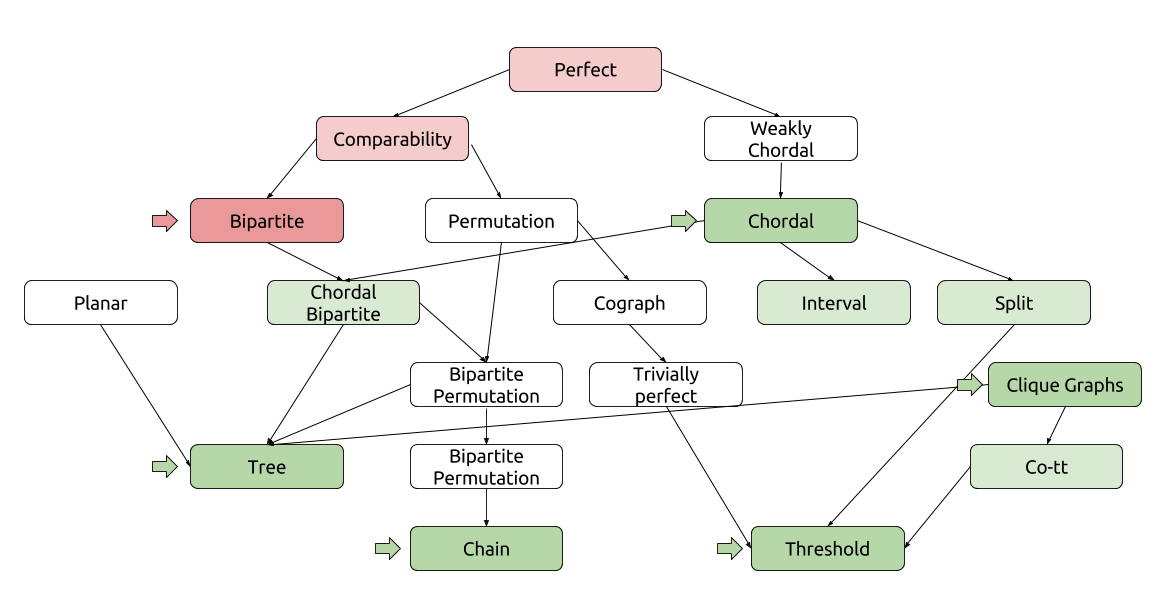
\includegraphics[width=18cm,center]{img/Figure2-1.png}
  \caption{
  Graph class inclusion graph: In red, classes proven NP-complete for the problem; In green, classes with polynomial algorithms. In red and light green, classes that are contained / contain other classes, consequently have the same results. Open classes are blank, with no definite result as to their complexity.}
  \label{fig:graph2}
\end{figure}

Or, for clarity on the results shown in the previous figure, see Table \ref{tab:2} with the theoretical results of some classes of graphs, and the reference to the test article:
\begin{table}[!htbp]
\caption{Resultados do problema para algumas classes de grafos e suas referências} \label{tab:2}
\begin{center}
 \begin{tabular}{||c c c||} 
 \hline
 Classe & Complexidade & Referência \\ [0.5ex] 
 \hline\hline
 Árvores & Polinomial & \cite{centeno2011} \\ 
 \hline
 Cordal & Polinomial & \cite{centeno2011} \\ 
 \hline
 Bipartido & NP-completo & \cite{Reddy2010} \\
 \hline
 \textit{Chain} & Polinomial &  \cite{Reddy2010}  \\
 \hline
 \textit{Threshold} & Polinomial & \cite{chen2009}\\
 \hline
 Clique & Polinomial & \cite{Nichterlein2013} \\
 \hline
\end{tabular}
\end{center}
\end{table}

As we can see, these results show how the treewidth strongly defines the difficulty of our problem.  


%Convex hull for P3  https://www.sciencedirect.com/science/article/pii/S1571065313002333
% parametrized stuff
%  * http://www.akt.tu-berlin.de/fileadmin/fg34/publications-akt/tss-long.pdf
%  * https://arxiv.org/pdf/1610.07530.pdf

% model with no results: https://link.springer.com/content/pdf/10.1007/s10878-018-0256-z.pdf
%model to maximize number of infected at the end: http://journals.tubitak.gov.tr/elektrik/issues/elk-18-26-6/elk-26-6-46-1802-212.pdf

% paper to beat. Has instances and concrete model. https://link.springer.com/content/pdf/10.1007/s10479-018-3107-5.pdf \cite{Soltani2019}

% M campelo work https://sol.sbc.org.br/index.php/etc/article/view/3176/3138

%Solução grande??????? Pedir vinicius  https://www.sciencedirect.com/science/article/pii/S1571065313002485#!
\begin{itemize}
\item Add images from presentation and organize as story
\end{itemize}

%Convex hull for P3  https://www.sciencedirect.com/science/article/pii/S1571065313002333
% parametrized stuff
%  * http://www.akt.tu-berlin.de/fileadmin/fg34/publications-akt/tss-long.pdf
%  * https://arxiv.org/pdf/1610.07530.pdf

% model with no results: https://link.springer.com/content/pdf/10.1007/s10878-018-0256-z.pdf
%model to maximize number of infected at the end: http://journals.tubitak.gov.tr/elektrik/issues/elk-18-26-6/elk-26-6-46-1802-212.pdf

% paper to beat. Has instances and concrete model. https://link.springer.com/content/pdf/10.1007/s10479-018-3107-5.pdf \cite{Soltani2019}

% M campelo work https://sol.sbc.org.br/index.php/etc/article/view/3176/3138

%Solução grande??????? Pedir vinicius  https://www.sciencedirect.com/science/article/pii/S1571065313002485#!

\chapter{Problem Formulations}

\section{Problem definition}

In a graph, an irreversible conversion process refers to the spreading of a characteristic through the graph, later referred here as an infection, where we have information on the stage of this process at each instant of time.  
Given a graph $G = (V, E)$, this process will be analyzed as a sequence of binary labels that determines if a particular vertex in that instant of time is active or inactive
\begin{equation}
c_{t}: V(G) \rightarrow \{0,1\}
\end{equation}
\begin{equation}
C = (c_{0}, c_{1} \dots )= (c_{t \in \mathbb{N}})
\end{equation}
The way the characteristic spreads through the graph is controlled by a threshold function $ f $, or later refereed here as the vertices' resistance, is defined as:
\begin{equation}
f: V (G) \rightarrow \mathbb{Z}^+.
\end{equation}

Now, given an initial graph where each vertex has a resistance to the "infection", if we have a initial subset of vertices in this graph that will start carrying the infection, an uninfected vertex will be infected if the total of its already infected neighbors surpasses the vertex's resistance. More formaly, given a $ G $ graph and a threshold function $ f $, the process begins with an initial binary labeling $ c_{0} $ of the vertices, while the rest of the labels are iteratively defined so that $\forall t \in \mathbb{Z}^+, t > 0$ e  $\forall u \in V(G)$
\begin{equation}
c_{t}(u) = 1 \iff  c_{t-1}(u) = 1 \lor \sum_{v \in N_{G}(u)} c_{t-1}(v)  \geq f(u). 
\end{equation}

 %The main problem in this dissertation consists of, given an initial instance of graph and resistance function, what is the least number of vertices that need to be initially infected so to assure all the graph eventually will be completely infected. 


Figure \ref{fig: graph1} shows an example of an irreversible conversion process over time, with two vertices being initially infected.

\begin{figure}
  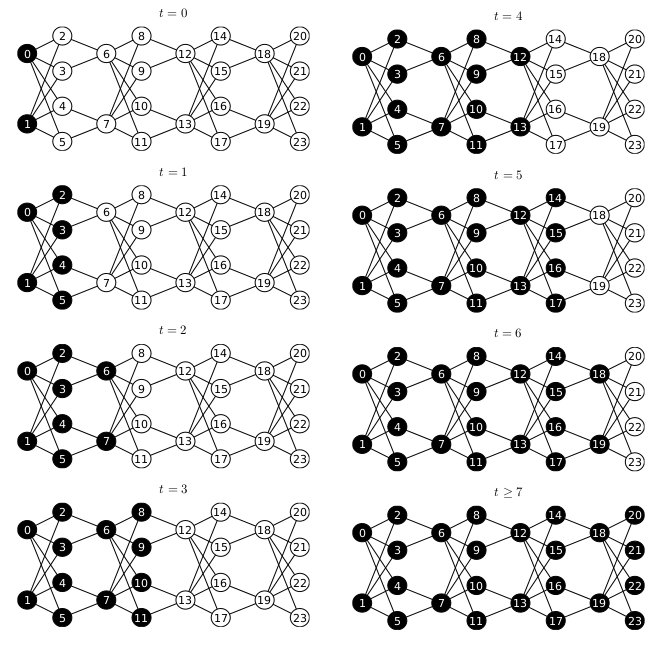
\includegraphics [width = \linewidth]{img/Figure3-1.png}
  \caption{Irreversible conversion process at different time points t for graph
of order 24, starting the process with convergent set and threshold function defined as $ f: V (G) \rightarrow {2}$. Source: \cite{amaral2015}}
  \label{fig: graph1}
\end{figure}

A convergent set is a label $ c_{0} $ which determines a certain sequence of labels $ c_ t$where

\begin{equation} 
\exists\ t_{s} \mid  v \in V(G) : c_{t_{s}}(v) = 1,
\end{equation}
and this set is denoted as
\begin{equation} 
\mathcal{C} = \{v \in V(G) : c_{0}(v) = 1\}
\end{equation}

  It follows from the definition that a trivial convergent set is $ V (G) $ itself. The minimum convergent set problem, or target set selection problem, is to find a convergent set as small as possible.

Given a constant threshold function $ f: V (G) \rightarrow \{k \}$ constant, \cite{centeno2011} has shown that this problem is NP-complete for any $ k \geq 2 $.

\section{Initial Formulation}

From these definitions, let the binary variable $ c_{t} (v) $ be the label of a vertex $ v $ in the instant $ t $ in our integer model.  $ c_{t} (v) = 1 $ will indicate if the vertex is infected (or active) and $ c_{t} (v) = 0 $ if not.

With this representation, it is evident that we want to minimize the number of infected tags at time 0, the initial infected vertices:
\begin{center}
\begin{equation}
min \sum_{v \in V} c_{0}(v)
\end{equation}
\end{center}


Also, for a workable solution to the problem, it is necessary to ensure that
\begin{center}
\begin{equation}
\begin{split} 
c_{t}(v) = 1 \iff c_{t-1}(v) = 1  \lor	 \sum_{\substack{ u \in \mathcal{N}_{G}(v) }} c_{t-1}(u) \geq f(v) \\ \\
\forall t \in 1, \ldots, |V|-1, v \in V 
\end{split}
\end{equation}
\end{center} 
which means that a vertex v has the label 1 (signiling it is infected) at a given instant t, then one of the following must be true:
\begin{itemize}
\item This vertex in the previous time instant was 1; or
\item In the previous time instant the number of infected neighbors of v surpassed f(v), threshold function of v.
\end{itemize}


Below, we separate the previous implication in multiple parts and translate them into linear restrictions that will have the same meaning in the model.

To represent the restriction that a label is infected at instant $ t $ implies that it is at the instant $ t + 1 $, that is
\begin{equation}
c_{t-1}(v) \implies c_{t}(v)
\end{equation}
we will use the constraint
\begin{equation}
c_{t-1}(v) \leq c_{t}(v).
\end{equation}
And the other part of our implication 
\begin{equation}
\sum_{\substack{ u \in \mathcal{N}_{G}(v) }} c_{t-1}(u) \geq f(v)  \implies c_{t}(v)
\end{equation}
can be described as
\begin{equation}
\sum_{u \in \mathcal{N}_{G}(v)}c_{t-1}(u) - f(v) + 1 \leq |V|c_{t}(v)  
\end{equation}
Now to show the implication back, that is
\begin{equation}
c_{t}(v) = 1 \\ \implies c_{t-1}(v) = 1 \lor	 \sum_{\substack{ u \in \mathcal{N}_{G}(v) }} c_{t-1}(u) \geq f(v)  
\end{equation}
or its contrapositive
\begin{equation}
c_{t-1}(v) == 0  \land \sum_{\substack{ u \in \mathcal{N}_{G}(v) }} c_{t-1}(u) < f(v) \\ \implies c_{t}(v) = 0  
\end{equation}
we have the following representation
\begin{equation}
\sum_{u \in N_{G}(v)}c_{t-1}(u) + f(v) \cdot c_{t-1}(v) \geq f(v) \cdot c_{t}(v) 
\end{equation}
Finally, so that all vertices are infected at the end of the process:
\begin{equation}
\sum_{v \in V}c_{|V| - 1}(v) = |V|   
\end{equation}
Notice that the process, in this case, will take at most $ | V | $ iterations to converge to its final state.
 Thus, the complete modeling of the problem is given below.
 
 
\begin{alignat*}{3}
    \text{minimize }   & \displaystyle\sum\limits_{v \in V} c_{0}(v)\  \\
    \text{subject to} \\ %& c_{t-1}(v) \leq c_{t}(v),  &t= \{1 .. |V|- 1\}, v \in V\\
&\displaystyle\sum\limits_{u \in \mathcal{N}_{G}(v)}c_{t-1}(u) - f(v) + 1\leq |V|c_{t}(v),  &t=\{1 .. |V|- 1\}, v \in V\\
&\displaystyle\sum\limits_{u \in N_{G}(v)} c_{t-1}(u) + f(v) \cdot c_{t-1}(v) \geq f(v) \cdot  c_{t}(v),  &t=\{1 .. |V|- 1\}, v \in V \\
&\displaystyle\sum\limits_{    v \in V}c_{|V| - 1}(v) = |V|  \\
& c_{t}(v) \in \{0,1\}, &t= \{1 .. |V|- 1\}, v \in V
  \end{alignat*}

\section{Formulations in the literature}
First, we analyse \cite{Ackerman2010}, that shows a formulation based on the idea that Target Set Selection is equivalent to constructing an acyclic tournament with the minimum number of sources (vertices $s \in V$ with $deg_{in}(s) = 0$).
Given a graph $G=(V,E)$, to define this model, first binary variable for each edge and non edge are created. % $E \cup E'$, where $E' = \{(u,v) | (u,v) \notin E\}$. 
    \begin{alignat*}{3}
        & e_{uv} \in \{0,1\}%   \textit{,   } (u,v) \in E \cup E' 
    \end{alignat*}
    And $s_v$ encodes whether v is infected initially.
    \begin{alignat*}{3}
        & s_v \in \{0,1\}\textit{,   } v \in V 
    \end{alignat*}
    
    At the end, the variables $e_{uv}$ selected determine a tournament (acyclic complete digraph) 
    \begin{alignat*}{3}
        e_{uv} + e_{vw} + e_{wu} \leq 2  \\
        e_{uv} + e_{vu} = 1 \\
        %\textit{distinct }u, v,  w \in V  
    \end{alignat*}
    Enforcing that a vertex that cannot be infected by others is selected in $s_v$
    \begin{alignat*}{3}
        \displaystyle\sum\limits_{(u, v) \in E} e_{uv} \geq t_v . (1 - s_v) \textit{,   } v \in V
    \end{alignat*}

This model is very important when studying the target set selection problem, but it does not have experimental results. Fortunately, we found \cite{Soltani2019}, where the corresponding 0–1 polytope and its facets are studied and several families of facet defining inequalities are introduced, but also computational experiments have been performed to show the strength of the IP formulation and its facet defining inequalities. Also, \citeauthor{Soltani2019} make their code available, which facilitates the comparison with our model.

\begin{itemize}
    \item Add figures: Model direct edges. Model with facet cutting inequalities 
    \item Maybe add detailed explanation from paper about constraints introduced in \cite{Soltani2019}
\end{itemize}

\chapter{Our Integer Model}
\section{Problem reductions}
Before presenting our formulation, some more direct reduction should be presented, not only to decrease the problem, but because they are also necessary for our new formulation to be correct.

\begin{myred}
    For a Target Set Selection instance $\mathcal{I} = \{G = (V,E), f\}$, and any $v \in V$ where $f(v) > \mathcal{N}_{G}(v)$, delete $v$, decrease the neighbors' threshold by one, and already add $v$ to the set of vertices that have to be initially infected.
\end{myred}

This reduction puts vertices that have to be in the minimum target set to infect the whole graph. In the following subsections, we will assume that the instances we are working with have all vertices with $\text{deg}(v) \geq f(v), \text{for} v \in V$, being necessary to prove properties we will use in the formulation.

\begin{figure}[!ht]
    %\newlength{\tempheight}
    %\setlength{\tempheight}{15ex}
    \centering
    \begin{subfigure}[t]{0.5\textwidth}
        \centering
         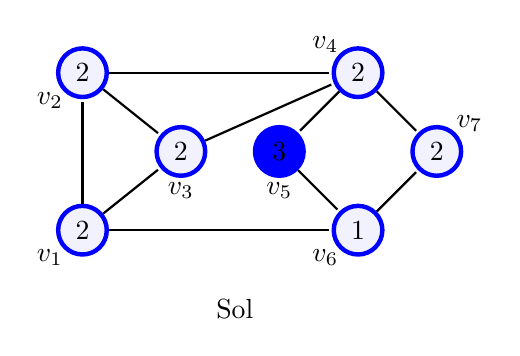
\begin{tikzpicture}[shorten >=1pt, auto, node distance=3cm, ultra thick]
    \tikzstyle{node_style} = [circle,draw=blue,fill=blue!5!]
    \tikzstyle{node_infected} = [circle,draw=blue,fill=blue!100!]
    \tikzstyle{edge_style} = [draw=black, line width=2, thick]
    \node[node_style] (v1) at (-2,-1) {2};
    \node[node_style] (v2) at (-2,1) {2};
    \node[node_style] (v3) at (-0.75,0) {2};
    \node[node_style] (v4) at (1.5,1) {2};
    \node[node_infected] (v5) at (0.5,0) {3};
    \node[node_style] (v6) at (1.5,-1) {1};
    \node[node_style] (v7) at (2.5,0) {2};
    
    \node[text width=2cm] at (0.7,-2) {Sol };
    \node [below left=3] at (v2) {$v_2$};
    \node [below left=3] at (v1) {$v_1$};
    \node [below=7] at (v3) {$v_3$};
    \node [above left=3] at (v4) {$v_4$};
    \node [below=7] at (v5) {$v_5$};
    \node [below left=3] at (v6) {$v_6$};
    \node [above right=3] at (v7) {$v_7$};

    
    \draw[edge_style]  (v1) edge (v2);
    \draw[edge_style]  (v1) edge (v3);
    \draw[edge_style]  (v2) edge (v3);
    \draw[edge_style]  (v1) edge (v6);
    \draw[edge_style]  (v2) edge (v4);
    \draw[edge_style]  (v3) edge (v4);
    \draw[edge_style]  (v4) edge (v5);
    \draw[edge_style]  (v5) edge (v6);
    \draw[edge_style]  (v4) edge (v7);
    \draw[edge_style]  (v6) edge (v7);
    \end{tikzpicture}
        \caption{Graph where the threshold value is inside each vertex. Notice that $\text{deg}(v_5) < f(v_5)$. We can use Reduction 1 in this Target Set Selection instance.}
        \label{fig:411}
    \end{subfigure}
    \begin{subfigure}[t]{0.5\textwidth}
        \centering
        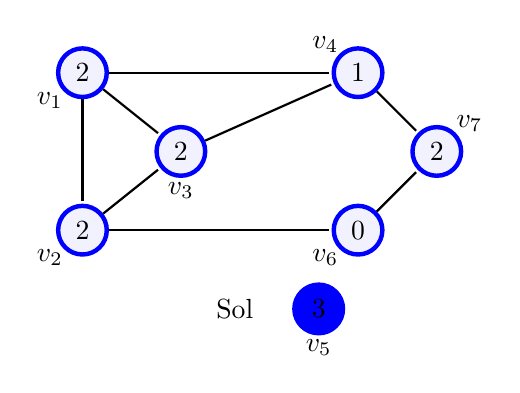
\begin{tikzpicture}[shorten >=1pt, auto, node distance=3cm, ultra thick]
    \tikzstyle{node_style} = [circle,draw=blue,fill=blue!5!]
    \tikzstyle{node_infected} = [circle,draw=blue,fill=blue!100!]
    \tikzstyle{edge_style} = [draw=black, line width=2, thick]
    \node[node_style] (v1) at (-2,1) {2};
    \node[node_style] (v2) at (-2,-1) {2};
    \node[node_style] (v3) at (-0.75,0) {2};
    \node[node_style] (v4) at (1.5,1) {1};
    \node[node_infected] (v5) at (1,-2) {3};
    \node[node_style] (v6) at (1.5,-1) {0};
    \node[node_style] (v7) at (2.5,0) {2};
    
    \node[text width=2cm] at (0.7,-2) {Sol };
    \node [below left=3] at (v2) {$v_2$};
    \node [below left=3] at (v1) {$v_1$};
    \node [below=7] at (v3) {$v_3$};
    \node [above left=3] at (v4) {$v_4$};
    \node [below=7] at (v5) {$v_5$};
    \node [below left=3] at (v6) {$v_6$};
    \node [above right=3] at (v7) {$v_7$};
    
    \draw[edge_style]  (v1) edge (v2);
    \draw[edge_style]  (v1) edge (v3);
    \draw[edge_style]  (v2) edge (v3);
    \draw[edge_style]  (v2) edge (v6);
    \draw[edge_style]  (v1) edge (v4);
    \draw[edge_style]  (v3) edge (v4);
    \draw[edge_style]  (v4) edge (v7);
    \draw[edge_style]  (v6) edge (v7);
    \end{tikzpicture}
        \caption{Instance resulting after applying Reduction 1 in the instance of Figure \ref{fig:411}}
        \label{fig:412}
    \end{subfigure}
\end{figure}

\begin{myred}
    For a Target Set Selection instance $\mathcal{I} = \{G = (V,E), f\}$,  and any $v \in V$ where $f(v) = 0$, delete $v$ and decrease thresholds. $v$ will not be in the solution.
\end{myred}
Also, we will need that for the whole graph, $f(v) > 0, v \in V$ as well.

\begin{figure}[!ht]
    %\setlength{\tempheight}{15ex}
    \centering%
    \begin{subfigure}[t]{0.5\textwidth}
        \centering%
         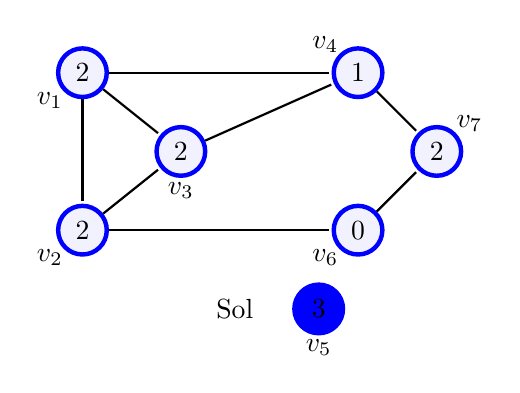
\begin{tikzpicture}[shorten >=1pt, auto, node distance=3cm, ultra thick]
    \tikzstyle{node_style} = [circle,draw=blue,fill=blue!5!]
    \tikzstyle{node_infected} = [circle,draw=blue,fill=blue!100!]
    \tikzstyle{edge_style} = [draw=black, line width=2, thick]
    \node[node_style] (v1) at (-2,1) {2};
    \node[node_style] (v2) at (-2,-1) {2};
    \node[node_style] (v3) at (-0.75,0) {2};
    \node[node_style] (v4) at (1.5,1) {1};
    \node[node_infected] (v5) at (1,-2) {3};
    \node[node_style] (v6) at (1.5,-1) {0};
    \node[node_style] (v7) at (2.5,0) {2};
    
    \node[text width=2cm] at (0.7,-2) {Sol };
    \node [below left=3] at (v2) {$v_2$};
    \node [below left=3] at (v1) {$v_1$};
    \node [below=7] at (v3) {$v_3$};
    \node [above left=3] at (v4) {$v_4$};
    \node [below=7] at (v5) {$v_5$};
    \node [below left=3] at (v6) {$v_6$};
    \node [above right=3] at (v7) {$v_7$};
    \draw[edge_style]  (v1) edge (v2);
    \draw[edge_style]  (v1) edge (v3);
    \draw[edge_style]  (v2) edge (v3);
    \draw[edge_style]  (v2) edge (v6);
    \draw[edge_style]  (v1) edge (v4);
    \draw[edge_style]  (v3) edge (v4);
    \draw[edge_style]  (v4) edge (v7);
    \draw[edge_style]  (v6) edge (v7);
    \end{tikzpicture}
        \caption{Graph where the threshold value is inside each vertex. Notice that $f(v_6) = 0$. We can use Reduction 2 in this Target Set Selection instance.}
        \label{fig:413}
    \end{subfigure}
    \begin{subfigure}[t]{0.5\textwidth}
        \centering
        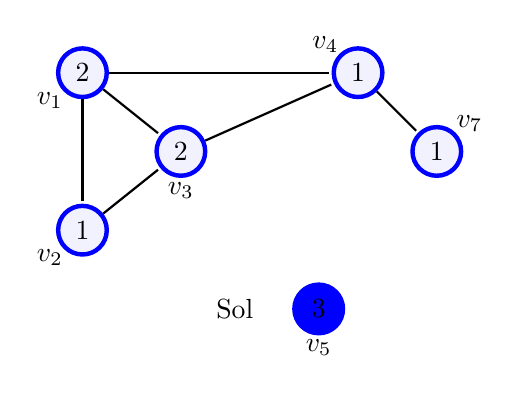
\begin{tikzpicture}[shorten >=1pt, auto, node distance=3cm, ultra thick]
    \tikzstyle{node_style} = [circle,draw=blue,fill=blue!5!]
    \tikzstyle{node_infected} = [circle,draw=blue,fill=blue!100!]
    \tikzstyle{edge_style} = [draw=black, line width=2, thick]
    \node[node_style] (v1) at (-2,1) {2};
    \node[node_style] (v2) at (-2,-1) {1};
    \node[node_style] (v3) at (-0.75,0) {2};
    \node[node_style] (v4) at (1.5,1) {1};
    \node[node_infected] (v5) at (1,-2) {3};
    \node[node_style] (v7) at (2.5,0) {1};
    
    \node[text width=2cm] at (0.7,-2) {Sol };
    \node [below left=3] at (v2) {$v_2$};
    \node [below left=3] at (v1) {$v_1$};
    \node [below=7] at (v3) {$v_3$};
    \node [above left=3] at (v4) {$v_4$};
    \node [below=7] at (v5) {$v_5$};
    \node [above right=3] at (v7) {$v_7$};
    
    \draw[edge_style]  (v1) edge (v2);
    \draw[edge_style]  (v1) edge (v3);
    \draw[edge_style]  (v2) edge (v3);
    \draw[edge_style]  (v1) edge (v4);
    \draw[edge_style]  (v3) edge (v4);
    \draw[edge_style]  (v4) edge (v7);
    \end{tikzpicture}
        \caption{Instance resulting after applying Reduction 2 in the instance of Figure \ref{fig:413}}
        \label{fig:414}
    \end{subfigure}
\end{figure}

\begin{myred}
    For a Target Set Selection instance $(G, f, Sol)$, reduced by Rule 1, and let  $v \in V (G)$ with $f(v) = \mathcal{N}_{G}(v) = 1$. Then, delete $v$ from $G$.
    \end{myred}
    An example for this reduction can be seen in Figure \ref{fig:415} and \ref{fig:416}.
Reduction 3 though will only help compressing our instances, being helpful in order to reduce the size of our problems, but not necessary in the next section proofs.


We can see an instance example in Figures \ref{fig:411} and the this instance reduced by Reduction 1 in \ref{fig:412}. Figures 
\ref{fig:413} and \ref{fig:414} show Reduction 2 and Figures \ref{fig:415} and \ref{fig:416} feature Reduction 3.

\begin{figure}[!ht]
    %\setlength{\tempheight}{15ex}
    \centering
    \begin{subfigure}[t]{0.4\textwidth}
        \centering
         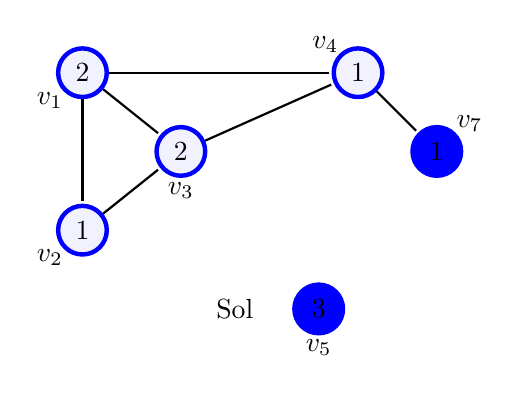
\begin{tikzpicture}[shorten >=1pt, auto, node distance=3cm, ultra thick]
    \tikzstyle{node_style} = [circle,draw=blue,fill=blue!5!]
    \tikzstyle{node_infected} = [circle,draw=blue,fill=blue!100!]
    \tikzstyle{edge_style} = [draw=black, line width=2, thick]
    \node[node_style] (v1) at (-2,1) {2};
    \node[node_style] (v2) at (-2,-1) {1};
    \node[node_style] (v3) at (-0.75,0) {2};
    \node[node_style] (v4) at (1.5,1) {1};
    \node[node_infected] (v5) at (1,-2) {3};
    \node[node_infected] (v7) at (2.5,0) {1};
    
    \node[text width=2cm] at (0.7,-2) {Sol };
    \node [below left=3] at (v2) {$v_2$};
    \node [below left=3] at (v1) {$v_1$};
    \node [below=7] at (v3) {$v_3$};
    \node [above left=3] at (v4) {$v_4$};
    \node [below=7] at (v5) {$v_5$};
    \node [above right=3] at (v7) {$v_7$};
    
    \draw[edge_style]  (v1) edge (v2);
    \draw[edge_style]  (v1) edge (v3);
    \draw[edge_style]  (v2) edge (v3);
    \draw[edge_style]  (v1) edge (v4);
    \draw[edge_style]  (v3) edge (v4);
    \draw[edge_style]  (v4) edge (v7);
    \end{tikzpicture}
         \caption{Graph where the threshold value is inside each vertex. Notice that $f(v_7) = \text{deg}(v_7) = 1$. We can use Reduction 3 in this Target Set Selection instance.}
        \label{fig:415}
    \end{subfigure}%
    \begin{subfigure}[t]{0.4\textwidth}
        \centering%
       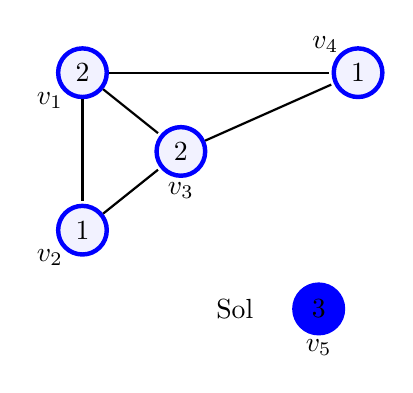
\begin{tikzpicture}[shorten >=1pt, auto, node distance=3cm, ultra thick]
    \tikzstyle{node_style} = [circle,draw=blue,fill=blue!5!]
    \tikzstyle{node_infected} = [circle,draw=blue,fill=blue!100!]
    \tikzstyle{edge_style} = [draw=black, line width=2, thick]
    \node[node_style] (v1) at (-2,1) {2};
    \node[node_style] (v2) at (-2,-1) {1};
    \node[node_style] (v3) at (-0.75,0) {2};
    \node[node_style] (v4) at (1.5,1) {1};
    \node[node_infected] (v5) at (1,-2) {3};
    
    
    \node[text width=2cm] at (0.7,-2) {Sol };
    \node [below left=3] at (v2) {$v_2$};
    \node [below left=3] at (v1) {$v_1$};
    \node [below=7] at (v3) {$v_3$};
    \node [above left=3] at (v4) {$v_4$};
    \node [below=7] at (v5) {$v_5$};
    
    \draw[edge_style]  (v1) edge (v2);
    \draw[edge_style]  (v1) edge (v3);
    \draw[edge_style]  (v2) edge (v3);
    \draw[edge_style]  (v1) edge (v4);
    \draw[edge_style]  (v3) edge (v4);
    \end{tikzpicture}
       \caption{Instance resulting after applying Reduction 3 in the instance of Figure \ref{fig:415}}
        \label{fig:416}
    \end{subfigure}
\end{figure}


\section{New formulation paradigm}

\subsection{General idea}

After analysing the previous introduced models, and defining some useful reductions in the previous sections, the idea was to get a model that would use some inherent property to the target set selection problem in order to improve its performance in more general graphs, since the previous models are said to perform better in sparse graph, more close to trees. With this in mind, we came up with a new paradigm to define this problem, based on the infection flow in a subset of vertices in the graph.

We will start by analysing one simple property that we know about the solution of a given instance of our problem.
\begin{myprop}
Given a Target Set Selection instance $ \mathcal{T} (G (V, E), f) $, where $G$ is our initial graph instance with set of vertices $V$ and edges $E$, and $f: V \to \mathbb{Z}^+$ our threshold function,  where Reductions 1 and 2 were applied. Then, a lower bound for the size of its Minimum Target Set is $\mathcal{C}$ is $\min_{v \ in V} f(v)$. 
\end{myprop},

\begin{proof}
This proof follows from the observation that, by contradiction, if you assume the number of initially infected vertices $|\mathcal{C}|$ are less then $ \min_{v \ in V} f(v) $,
since $f(v) \leq deg(v), \forall v \in V$, we know that $|\mathcal{C}| < \min_{v \ in V} f(v) \leq deg(v) < |V| $, we have that $\mathcal{C} \neq V$, so not all vertices are initially infected. Also, since $f(v) > 0, \forall v \in V$ no vertex will automatically infect itself. Now, we have that at least one vertex needs to be infected in order to spread the infection to the whole graph. So, we need $f(v) < |	\mathcal{C} \cap deg(v)|$ for some $v$. But $min_{v \in V} f(v) > |\mathcal{C}| \implies f(v) > |\mathcal{C}|, \forall v \in V \implies f(v) > |\mathcal{C} \cap deg(v)|$. Contradiction.
\end{proof}

With this property, we tried to generalize it for a subset of $V$. So, if $S \subset V$ was an isolated graph, we would know that for this set to be infected, at least $min_{v \in S}(f(v))$ vertices would have to infected at the beginning of the conversion process. When $S$ is not isolated from the rest of the graph, the difference are the edges between $S$ and $V \setminus S$ that can influence in the infection inside $S$. We know that these edges that go from $V \setminus S$ to $S$ can contribute to infect only the vertex they target with a "unit" of infection. We want to know at least how many vertices in $S$ would have to be infected at the beginning of the process in order to infect the whole subset. At least, all these edges will help infect $S$, and in this case each vertex would need to threshold function minus the number of edges coming from outside $S$,  $f(v) - |\mathcal{N}(v) \cap V \setminus S|$ to get infected, which means that $\min_{v \in V} |\mathcal{N}(v) \cap V \setminus S|$ is a lower bound for the vertices from $S$ that need to be in the target set solution. In the following section we prove this affirmation step by step.
 \begin{figure}[!ht]
    %\setlength{\tempheight}{15ex}
    \centering%
    \begin{subfigure}[t]{0.5\textwidth}
        \centering%
        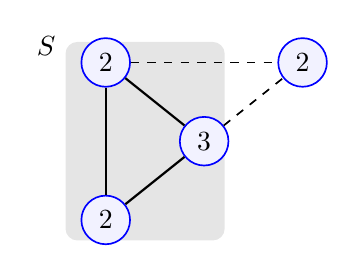
\begin{tikzpicture}[
    auto, % automatic node positioning
    node distance=2cm,
    semithick,
    bend angle=10,
    graybox/.style = {draw=gray!20, fill=gray!20, rounded corners},
    line/.style = {-&gt;, draw=black, thick},
    box/.style = {circle, draw=blue!50, fill=blue!20, minimum size=4mm}
    ]
    \tikzstyle{node_style} = [circle,draw=blue,fill=blue!5!]
    \tikzstyle{node_infected} = [circle,draw=blue,fill=blue!100!]
    \tikzstyle{node_infected2} = [circle,draw=blue,fill=blue!40!]
    \tikzstyle{edge_style} = [draw=black, line width=2, thick]
    \node (BBox) [graybox, minimum width=2cm, minimum height=2.5cm] at (-1.5cm, 0cm) {};
    \node [left] at (BBox.130) {$S$};
    \node[node_style] (v1) at (-2,1) {2};
    \node[node_style] (v2) at (-2,-1) {2};
    \node[node_style] (v3) at (-0.75,0) {3};
    \node[node_style] (v4) at (0.5,1) {2};
    
    \draw[edge_style]  (v1) edge (v2);
    \draw[edge_style]  (v1) edge (v3);
    \draw[edge_style]  (v2) edge (v3);
    \draw[dashed] (v1) edge (v4);
    \draw[dashed]  (v3) edge (v4);
    \end{tikzpicture}
        \caption{Instance where the threshold of each vertex is inside the node. Notice that the edges are between $S$ and $V \setminus S$.}
    \label{fig:416a}
    \end{subfigure}%
    \begin{subfigure}[t]{0.5\textwidth}
        \centering%
        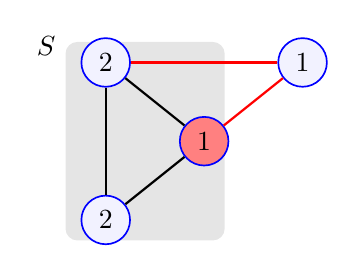
\begin{tikzpicture}[
    auto, % automatic node positioning
    node distance=2cm,
    semithick,
    bend angle=10,
    graybox/.style = {draw=gray!20, fill=gray!20, rounded corners},
    line/.style = {-&gt;, draw=black, thick},
    box/.style = {circle, draw=blue!50, fill=blue!20, minimum size=4mm}
    ]
    \tikzstyle{node_style} = [circle,draw=blue,fill=blue!5!]
    \tikzstyle{node_infected} = [circle,draw=blue,fill=red!50!]
    \tikzstyle{node_infected2} = [circle,draw=blue,fill=blue!40!]
    \tikzstyle{edge_style} = [draw=black, line width=2, thick]
    \tikzstyle{edge_dashed} = [draw=red, line width=4, thick]
    \node (BBox) [graybox, minimum width=2cm, minimum height=2.5cm] at (-1.5cm, 0cm) {};
    \node [left] at (BBox.130) {$S$};
    \node[node_style] (v1) at (-2,1) {2};
    \node[node_style] (v2) at (-2,-1) {2};
    \node[node_infected] (v3) at (-0.75,0) {1};
    \node[node_style] (v4) at (0.5,1) {1};
    
    \draw[edge_style]  (v1) edge (v2);
    \draw[edge_style]  (v1) edge (v3);
    \draw[edge_style]  (v2) edge (v3);
    \draw[edge_dashed] (v1) edge (v4);
    \draw[edge_dashed]  (v3) edge (v4);
    \end{tikzpicture}
        \caption{Thresholds were updated to their lower bound value $f(v) - | \mathcal{N}(v) \cap V \setminus S$. In this case, the lower bound for the target set size in $S$ is $min_{v \in S} f(v) - | \mathcal{N}(v) \cap V \setminus S = 1$.}
        \label{fig:416b}
    \end{subfigure}
\end{figure}
    %\centering{For $\mathcal{C}$ instance solution, $ |\mathcal{C} \cap S| \geq min_{v \in S} (f(v))$}

Based on this idea, we started to prove some properties regarding subsets $S$ of $V$.

\subsection{Graph Subset Properties}

Given an reduced instance $\mathcal{T}(G(V, E), f)$ as defined previously, in the Equation \ref{eq:2} we define the cut-set size as
  \begin{equation}\label{eq:2}
\delta(S) = |\{v_1v_2 \in E:  v_1 \in S , v_2 \in (V\setminus S)\} |
\end{equation}

Given a graph, a subset $S$, and minimum target set where the initial infected labels are given by $\mathcal{C}$, label that indicates if a vertex is infected $(1)$, or not $(0)$, we will be interested in sets $S$ where $\min_{v \in S} (f(v)) > \delta(S)$, so the following propositions can be proved.

\begin{myprop}
Given a set $S$ and $\mathcal{C}$,  %$\min_{v \in S} (f(v))$ and $\delta(S)$ as seen before, 
we have that
\begin{equation}
|\mathcal{C} \cap S | \geq \min_{v \in S} (f(v)) - \delta (S)
\end{equation}
\end{myprop}
%\footnote{não precisa nem $\min_{v \in S} (f(v))$ nem $\delta$ são operações já definidas }
\begin{proof} 
%This proof is simple.\footnote{tirar} 
First, we consider the case where every vertex in S is initially infected:
In this case, we know that $|\mathcal{C} \cap S | = |S|$. We also know that $f(v) \leq \mathcal{N}_G(v) $.  Besides, we notice that $\min_{v \in S} (f(v)) \leq f(v) \leq \mathcal{N}_G(v), v \in S$. So, if $ \delta(S)$ is the number of edges between $S$ and $V \setminus S$ . So, this implies that
\begin{equation}
\min_{v \in S} (f(v)) - \delta (S) \leq \mathcal{N}_G(v) \cap S  \leq |S| = |\mathcal{C} \cap S | 
\end{equation}
as we wanted to prove.

Now, suppose we have at least one vertex not infected at the beginning of the process. Let the first vertex of S %\footnote{of $S$}
to get infected after the process begins %\footnote{to get infected after the process begins} \footnote{como garante que esse vértice existe. Tem que excluir o caso em que todos os vértices de S estão infetados no começo} 
be $u$, where $u \notin C_0(S)$. We know that  $\min_{v \in S} (f(v)) \leq f(u)$ by definition of $\min_{v \in S} (f(v))$, and that $u$ can have, at most,  $\delta(S)$ infected neighbors outside $S$, so, to infect $u$, we need at least $f(u) -\delta(S)$. So, we know that, $|\mathcal{C} \cap S | \geq f(u) - \delta(S) \geq \min_{v \in S} (f(v)) - \delta(S) $.
\end{proof}

Let $\mathcal{N}_G(v)$ be the set of neighbors of a given vertex $v \in V(G)$.

\begin{myprop}
Given a set $S$,  $c_0$,  $\min_{v \in S} (f(v))$ and $\delta(S)$ as seen before, we have that 
\begin{equation}
|\mathcal{C} \cap S | \geq \min_{v \in S} (f(v)) - \max_{v \in S} (|\mathcal{N}_G(v) \cap (V \setminus S)|)
\end{equation}
\end{myprop}
\begin{proof}
As before, we consider two cases: 

First, we consider the case where every vertex in S is initially infected. We know that $|\mathcal{C} \cap S | = |S|$ and  $f(v) \leq \mathcal{N}_G(v) $.  Besides, we have that $\min_{v \in S} (f(v)) \leq f(v) \leq \mathcal{N}_G(v), v \in S$.  So, this implies that
\begin{gather}
\min_{v \in S} (f(v)) - \max_{v \in S} (|\mathcal{N}_G(v) \cap (V \setminus S)|) =\\
\min_{v \in S} (f(v))  - \max_{v \in S} (|\mathcal{N}_G(v) \cap (V \setminus S)|) \leq \\
f(v) - |\mathcal{N}_G(v) \cap (V \setminus S)| \leq \\ 
{N}_G(v)  - |\mathcal{N}_G(v) \cap (V \setminus S)| = \\ 
\mathcal{N}_G(v) \cap S  \leq\\  |S| = |\mathcal{C} \cap S | 
\end{gather}
as we wanted to prove.

Second, the case where at least one vertex was not infected in the beginning of the process. 
As before %\footnote{as before}%
, let $u \in S$ be the first vertex to be infected, where $u \notin C_0(S)$,    

$|{N}_G(u) \cap (V \setminus S)| \leq \max_{v \in S} (|\mathcal{N}_G(v) \cap (V \setminus S)|) \implies$ 

$\min_{v \in S} (f(v)) - |{N}_G(u) \cap (V \setminus S)| \geq \min_{v \in S} (f(v)) - \max_{v \in S} (|\mathcal{N}_G(v) \cap (V \setminus S)|) $.

Knowing that , by definition,  $f(u) \geq \min_{v \in S} (f(v))  \implies $ 

$f(u) - |{N}_G(u) \cap (V \setminus S)| \geq \min_{v \in S} (f(v)) - |{N}_G(u) \cap (V \setminus S)| \geq \min_{v \in S} (f(v)) - \max_{v \in S} (|\mathcal{N}_G(v) \cap (V \setminus S)|)  \implies$

$f(u) - |{N}_G(u) \cap (V \setminus S)|  \geq \min_{v \in S} (f(v)) - \max_{v \in S} (|\mathcal{N}_G(v) \cap (V \setminus S)|)  \implies$

%If $u$ was the first to be infected, we know that $|\mathcal{C} \cap S | \geq f(u) -  |{N}_G(u) \cap (V \setminus S)|$, since these are the only possibly infected neighbors of $u$\footnote{, 
Since $|{N}_G(u) \cap (V \setminus S)|$ is a maximum on the number of vertices outside $S$ that can help $u$ to become infected. Now, we have that:

$|\mathcal{C} \cap S | \geq f(u) - |{N}_G(u) \cap (V \setminus S)|  \geq \min_{v \in S} (f(v)) - \max_{v \in S} (|\mathcal{N}_G(v) \cap (V \setminus S)|)  \implies$

$|\mathcal{C} \cap S | \geq \min_{v \in S} (f(v)) - \max_{v \in S} (|\mathcal{N}_G(v) \cap (V \setminus S)|)$.

\end{proof}
\begin{mylemma}
Given a set $S$,  $|\mathcal{C} \cap S | $,  $\min_{v \in S} (f(v))$ and $\delta(S)$ as seen before, and we have that 
\begin{equation}
|\mathcal{C} \cap S | \geq  \min_{v \in S} (f(v) - |\mathcal{N}_G(v) \cap (V \setminus S)| ) 
\end{equation}
\end{mylemma}
\begin{proof}
If all vertices in $S$ were initially infected: Similar to the proof shown before,  for $v \in S$:
\begin{gather}
\min_{v \in S} (f(v) - |\mathcal{N}_G(v) \cap (V \setminus S)| ) \leq \\
f(v) - |\mathcal{N}_G(v) \cap (V \setminus S)| \leq \\ 
{N}_G(v)  - |\mathcal{N}_G(v) \cap (V \setminus S)| = \\ 
\mathcal{N}_G(v) \cap S  \leq |S| = \\
|\mathcal{C} \cap S | 
\end{gather}

proving this part of the proposition.
Now, for the case where at least one vertex was not initially infected.
We assume that  $|\mathcal{C} \cap S | <  \min_{v \in S} (f(v) - |\mathcal{N}_G(v) \cap (V \setminus S)|) $. We will prove that no $u \in S, u \notin C_0(S)$ can be infected.

Assume that $u \in S$ was the first vertex we attempted to infect, and $u \notin C_0(S)$. We want to proof that $|\mathcal{C} \cap S | + |\mathcal{N}_G(u) \cap (V \setminus S)| < f(u)$, no matter which $u$ is chosen, therefore we don't have a first vertex being infected.  
By hypothesis, we have:
\begin{center}
$|\mathcal{C} \cap S | <  \min_{v \in S} (f(v) - |\mathcal{N}_G(v) \cap (V \setminus S)|) \leq f(u) - |\mathcal{N}_G(u) \cap (V \setminus S)| \implies$

$|\mathcal{C} \cap S | <  f(u) - |\mathcal{N}_G(u) \cap (V \setminus S)| \implies$

$|\mathcal{C} \cap S | + |\mathcal{N}_G(u) \cap (V \setminus S)|<  f(u)$.
\end{center}
\end{proof}

\begin{mytheo} Given a Target Set Selection Instance $\mathcal{T}(G, f)$, $\mathcal{C} \subseteq V$ vertex set,   
\begin{equation}
\mathcal{C} \textit{ is convergent set in instance } \mathcal{T}(G, f) \iff |\mathcal{C} \cap S|\geq  \min_{v \in S} (f(v) - |\mathcal{N}_G(v) \cap (V \setminus S)| ) 
\end{equation}\end{mytheo} 
\begin{proof}
First, we proved the implication $\mathcal{C} \implies |\mathcal{C} \cap S| \geq  \min_{v \in S} (f(v) - |\mathcal{N}_G(v) \cap (V \setminus S)| )  $in the previous lemma. 

For the implication's other direction, assuming $\mathcal{C}$ is not convergent, we will prove that exists at least one $S$ where $|\mathcal{C} \cap S| <  \min_{v \in S} (f(v) - |\mathcal{N}_G(v) \cap (V \setminus S)| )  $. $\mathcal{C}$ is not convergent,  which means that if we simulate the spread of infection through the graph, not all vertices are infected. Take this set of infected vertices as $S$. 

Now we know that $ |\mathcal{C} \cap S| = 0 < \min_{v \in S} (f(v) - |\mathcal{N}_G(v) \cap (V \setminus S)| )$, otherwise, if for any $u \in S, f(u) - |\mathcal{N}_G(u) \cap (V \setminus S)| \leq 0 \implies f(u) \leq   |\mathcal{N}_G(u) \cap (V \setminus S)|$, which means $u$ would have been infected by the vertices outside $S$, contradiction.
\end{proof}


\subsection{Model and Constraints Found}

Based of the theorem previosly shown, we know, we know that if we find $\mathcal{C}$ convergent set, then any subset $S \subseteq V$ should hold for the inequality
\begin{equation}
    |\mathcal{C} \cap S| \geq \min_{v \in S} (f(v) - |\mathcal{N}_G(v) \cap (V \setminus S)| ) 
\end{equation}
We will be using this to define our model, where first we provide an empty $\mathcal{C}$. We will find an $S$ that violates equation , which means
\begin{equation}
    |\mathcal{C} \cap S| < \min_{v \in S} (f(v) - |\mathcal{N}_G(v) \cap (V \setminus S)| ) 
\end{equation}
When $\mathcal{C}$ is empty, if $S $
\begin{myprop}
For any $\mathcal{C}$ possible target set, if $|S| = 1$, than $S$ does not define a violated inequality.
\end{myprop}
\begin{proof}
Considering the premises guaranteed, we know that $\mathcal{N}_G(v) \geq f(v), v \in V$. With $S = \{v\}$, we have that

$\min_{v \in S} (f(v) - |\mathcal{N}_G(v) \cap (V \setminus S)| ) = f(v) - N_G(v)  < 0$ 

implying  that the inequality is never violated, since the following is always true:  

$|\mathcal{C} \cap S | \geq 0 \geq\min_{v \in S} (f(v) - |\mathcal{N}_G(v) \cap (V \setminus S)|) $ 
\end{proof}

\begin{myprop}
Given an $S$ that does not induce a connected graph, and $S$ generates a violated inequality, then exist an a $S' \subset S$, such that $S'$ induce a connected graph and $|\mathcal{C} \cap S | <  \min_{v \in S'} (f(v) - |\mathcal{N}_G(v) \cap (V \setminus S')|) $ will generate a violated inequality
\end{myprop}
\begin{proof}
Here, we first find the $v = \text{argmin}_{v \in S} (f(v) - |\mathcal{N}_G(v) \cap (V \setminus S)|)$. This $v$ is in a connected component in $S$, lets call it $S'$. It follows that $|\mathcal{C} \cap S' | \leq |\mathcal{C} \cap S | <  \min_{v \in S'} (f(v) - |\mathcal{N}_G(v) \cap (V \setminus S')|) $, proving $S'$ does also define a violated inequality. 
\end{proof}

\begin{myprop}
$ | N_G(v) \cap \mathcal{C}|  \geq f(v) \implies v \neq \text{argmin} (f(v) - |N_G(v) \cup V\setminus S|)$ , for $\forall S \subset V$
\end{myprop}
\begin{proof}
<Don't know what this proposition meant.>
\end{proof}

Write here algorithm that: starts infecting 1 vertex. Starts the process. If the process won't stop, create a violated inequality where S is the set of vertices that has not been infected. Do it till you infect all graph. This will generate a optimal solution for the problem here.
\begin{myprop}
This algorithm generates a model for the problem PCP
\end{myprop}
\begin{proof}

\end{proof}
Based on this results, create heuristic based on Prim's algorithm that creates S's based on a greedy choice 


After the results previously shown, that guarantee properties of any given $S$ set of vertices and $c_0$ solution to the target set selection problem, we can derive that, given a integer solution to the initial given model, if the properties proven above hold, then we have a viable solution, otherwise, if we find an S that does not hold that property, immediately we can derive a new constraint to our problem. We will name this constraint, our violated inequalities, that will be added to the model, and guarantee the model converges to the optimal solution.

%\section{Constraints}

%\section{Model}


\chapter{Branch-and-cut algorithm and Separation problem}

\section{Lazy Reformulation}
Say all models we tried to use, all variations of the problem. What is the problem with each and every one. And what we deemed the best


\section{NP-completeness}

Based on the previous findings, we showed that violated inequalities are found, given an integer solution to the previous integer problem.  A problem we have here is that , to find a integer solution, a solver can take a considerable amount of time. Having this in mind, a possible way of accelerating our problem finding is to use the linear solutions found in the middle time, in the process of branch and bounding that are necessarily to find the the integer solution. In order to find violated inequalities based on a solution to the relaxation version of the problem, we have to solve the separation problem, which can be defined as follows:
%\begin{mydef}[Violated inequality]
%Given a solution to the relaxation target set problem $c_0(V) = \{ x_0, ..., x_{n-1} \}$, where each $x_i \in [0,1]$,  find a violated inequality.
% \end{mydef}

\begin{mydef}[Separation problem]
Given a solution to the relaxation target set problem $c_0(V) = \{ x_0, ..., x_{n-1} \}$, where each $x_i \in [0,1]$,  find if there is an $S \subseteq V$, where   
\begin{equation}
c_0^{-1}(S) <  \min_{v \in S} (f(v) - |\mathcal{N}_G(v) \cap (V \setminus S)| ) 
\end{equation}
\end{mydef}

This problem can be generalized to :
\begin{mydef}[Minimum Infected Subset]
Given a graph $G = (V, E)$,  function $f: V\rightarrow \mathbb{N}$  threshold, and a function,  $x: V \rightarrow [0, 1]$ , find if there is an $S \subseteq V$, where   
\begin{equation}
 \displaystyle\sum\limits_{v \in S} x(v)   <  \min_{v \in S} (f(v) - |\mathcal{N}_G(v) \cap (V \setminus S)| ) 
\end{equation}
\end{mydef}

We proved that this problem is NP-complete, by reducing the Exact Cover by 3 to this problem, based on the work of \citep{Araujo2018}, where the reduction used inspired the reduction to our , then, open problem.
\begin{mydef}[Exact Cover by 3]
Given a family $\mathcal{F} = \{f_1, ..., f_m\}$, where each $f_i $ is a set with three elements, and a family $\mathcal{X}$ of $3n$ elements, where $m > n$. Is there an exact cover of $\mathcal{X}$ by $\mathcal{F}$ (where each element of $\mathcal{X}$ is only cover by  one $f_i$ , and each $f_i$ covers 3 elements of $\mathcal{X}$)?
\end{mydef}


\begin{mytheo}[Reduction from Exact cover by 3 to Minimum infected subset]
Given an instance of the exact cover by 3 problem, we can build an instance to our problem, where, we have a Yes answer for this constructed instance, if and only if we will have a Yes answer for the original instance.  
\end{mytheo}
\begin{proof}
First, we will consider an instance of Exact Cover by 3 problem $(\mathcal{F}, \mathcal{X})$, where $|\mathcal{F}| = m, |\mathcal{X}| = 3n$. A graph $G = (V, E)$ can be constructed as the shown in Figure \ref{fig:reduction}. The vertices created correspond to: 
\begin{itemize}
\item $A_i$: one vertex per $f_i \in \mathcal{F}$;
\item $B_i$ : one vertex per $x_i \in \mathcal{X}$; 
\item $W$, $U'$ and $U''$ auxiliary vertices;  
\end{itemize}
For each vertex $A_i$, we create one edge $\{A_i, W\}$ and three edges $\{Ai, Bj\}$, where $x_j \in f_i$. For each vertex $B_i$, create the edges $\{B_i, U'\}$  and $\{B_i, U''\}$. Finally, the edges $\{U', W\}$ and $\{U'', W\}$ are added to the graph. We define the threshold function $f(v) = 2$, and $w(v) = \frac{1}{m + 2n + 2} -  \epsilon $, where $\epsilon < < 1$. 

$\Rightarrow$ Prove that an Yes instance for the Exact Cover by 3-sets implies an Yes instance for the  Minimum Infected Subset for the constructed graph:

Let $\mathcal{F}' \subseteq \mathcal{F}$ be the correspondent exact cover for the given instance. Correspondent to $\mathcal{F}'$ we have $\mathcal{A}'  \subseteq \mathcal{A}$, vertices corresponding to the selected sets in $\mathcal{F}'$. Let $\overline{S} = A' \cup \{U\} \cup \{W\}$, we show that $ \displaystyle\sum\limits_{v \in S} w(v)   <  2 -  \min_{v \in S} |\mathcal{N}_{\overline{S}}(v)| $. 
\begin{itemize}
\item For $A_i \in S$: $A_i \notin A'$ , so $|\mathcal{N}_{\overline{S}}(A_i)| = \{w\}$;
\item For $B_i \in S$: $B_i \in B'$ , and  $|\mathcal{N}_{\overline{S}}(B_i)| = \{A_j\}$, where $A_j \in A'$, which is unique, since $A'$ is an exact cover;
\item For $U', U'' \in S$: $|\mathcal{N}_{\overline{S}}(U')| =  |\mathcal{N}_{\overline{S}}(U'')| = \{w\}$.
\end{itemize}
Which means that $\min_{v \in S} |\mathcal{N}_{\overline{S}}(v)|  = 1$, at most. And we have $ \displaystyle\sum\limits_{v \in S} w(v) = (m + 2n +2) . (\frac{1}{m + 2n + 2} - \epsilon)  = 1 - \epsilon < 2 - 1 = 1$. \\

\par
$\Leftarrow$ Prove that an Yes instance for the  Minimum Infected Subset implies an Yes instance for the Exact Cover by 3-sets  for the constructed graph:

We have  an $S \subseteq V $ where $ \displaystyle\sum\limits_{v \in S} w(v)   <  2 -  \min_{v \in S} |\mathcal{N}_{\overline{S}}(v)|$, we will show that  $\overline{S} = A' \cup \{W\}$.
The problem can not return an empty S, so, we have at least 1 vertex in S. So, it can not be only W, since $|\mathcal{N}_{\overline{S}}(W)| = |\{A\}| = m > 1$, it can not be one $A_i \in A$, since $|\mathcal{N}_{\overline{S}}(A_i)| = 3 > 1$, and it cannot be any $B_i \in B$ because 
First, assume that $U', U'' \in \overline{S}$. This implies that $\forall B_i \in B$, if $B_i \in S$,   $|\mathcal{N}_{\overline{S}}(B_i)| = \{U', U''\}$. So, only if all $B \subseteq \overline{S}$, but in that case each $|\mathcal{N}_{\overline{S}}(A_i)| = 3$, so  $A \subset \overline{S}$, but consequently W has to be in $\overline{S}$. S would be empty. 
 
 Without loss of generality, assume $U' \in \overline{S}$. This implies that if any $B_i \in \overline{S}$, $|\mathcal{N}_{\overline{S}}(U'')| = \{U', B_i\}$. So $B \subset S$. If any $A_i \in \overline{S}$, we have that exist $B_j$, where $|\mathcal{N}_{\overline{S}}(B_j)| = \{U', A_i\}$. So $A \in S$. Which means that$ \displaystyle\sum\limits_{v \in S} w(v)  >= ( m + 3n + 1 ) \frac{1}{m + 2n + 2} > 1 $. S has to much weight to be valid.

Now we know that both $U', U'' \in S$. In order to $S$ not overload, we need to take out of $S$ at least $n + 1$ vertices.

If $W \in S$, we could not have at most one  $A_i \in \overline{S}$, which means that we would have at most 3 vertices $B_j$ covered only by this $A_i$ . Meaning that S will become overloaded again with $(m + 3(n - 1) + 2)$ vertices in S.  
Now, with $W \in \overline{S}$, we have to take out of $S$ at least n vertices.
No $B_i$ can be taken out of $S$, since otherwise we would have $|\mathcal{N}_{\overline{S}}(U')| = |\{B_i, W\} | = 2$.
Let $A'' \subset A$, where $A'' \subset \overline{S}$ and $|A''| = n$ at least. We know that $\bigcap_{A_i \in A''} A_i = \emptyset$, otherwise if $\exists A_i, A_j \in A'', A_i \cap A_j = \{ B_k\} \implies |\mathcal{N}_{\overline{S}}(B_k)| = |\{A_i, A_j\}| = 2 $. This shows as well that $|A''| = n$. This shows that this found $A''$ is correspondent to an exact cover by 3-sets to the original instance.
\end{proof}
\begin{figure}
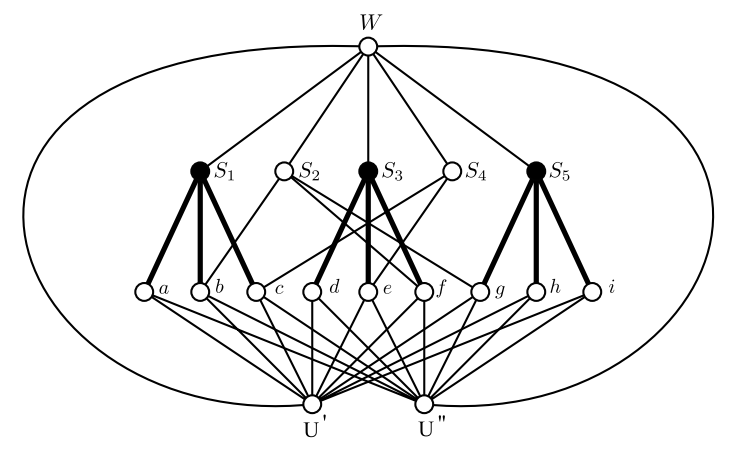
\includegraphics[width=14cm]{img/Figure6-1.png}
\caption{Reduction of Exact Cover by 3-sets to the Minimun Infected Subset. Image source: \cite{Araujo2018}}
\label{fig:reduction}
\end{figure}



\section{Heuristics}
Initial constraints created: the reductions and the one based on the pair of vertices
Initial approach: list all possible S's. Problem 
After, basic greedy heuristic was tried;
Cluster HCS ideia

\section{Instances used and implemented}
Here, describe the coloring problem instances and how instances were build, and the ones based on the paper \citet{raghavan2015}


\chapter{Experimental Results}
\input{chapter/ExperimentalResults.tex}

SUMMARY OF WHAT TO DO NEXT
Paper regarding p3 convexity and find instances to compare 

See if Chinese paper was published: was published

find code and see how it finally is. Retest with all the possible heuristic to find spread disease, make table and compare results

Finally, get best and compare with literature: Have to discover instances in literature to compare with here.

Try to extract paper in the progress and make presentation at the same time, since images for presentation should be used in dissertation.


Learn about cplex configurations and start tuning it to better model and explain in presentation. Also remember concepts like lazy constraints against other possible constraints

The House of Graphs: creates graph instances 


After Vinicius meeting
Make slides for next week
Get all references in whatsapp and use them in the results
Use paper on convexity p3 in the dissertation, add section on convexity and so on, since is the problem we can solve  with ease. 

\chapter{Conclusion}
\input{chapter/Conclusion.tex}

\ppgccbibliography{bibfile.bib}



\end{document}
